\section{引言}

四维 $\cN{=}2$ 超对称量子场论的研究，长期以来一直是理论物理学家耕耘的一片沃土。这些理论中的物质场表示总是非手征的，因此永远不可能直接用于描述真实世界。尽管如此，两组超对称性的存在，使我们能够比在非超对称理论或 $\cN{=}1$ 超对称理论中更为细致地研究它们的性质。能够进行这样的研究，本身就颇有乐趣；而且，我们希望由此获得的有关 $\cN{=}2$ 超对称理论的一般性认识，在研究超对称性较少的理论的动力学时也会有所帮助。至少，人们已经成功地利用 $\cN{=}2$ 理论的物理性质，向数学家揭示了若干他们此前并不知道的新数学现象。

这些话大概还不足以说服原本缺乏兴趣的人开始研究 $\cN{=}2$ 动力学。不过，作者并不打算在这里提出一套令人信服的论证，来说明你为什么无论如何都应当研究它；既然你正在阅读这句话，就应当意味着你已经对这个主题有些兴趣，而且正在寻找一个入门之处。

自 $\cN{=}2$ 理论提出以来\cite{Fayet:1975yi}，这一领域已经出现了许多重要贡献。依作者非常个人化的看法，其中最重要的四项如下：
\begin{itemize}
\item 1994 年，Seiberg 和 Witten 在文献\cite{Seiberg:1994rs,Seiberg:1994aj}中利用全纯性，并引入 Seiberg-Witten 曲线的概念，找到了 $\cN{=}2$ 超对称 $\SU(2)$ 规范理论的精确低能解。
\item 1996--1997 年，此前一直作为数学辅助对象的 Seiberg-Witten 曲线，被认定为 $\cN{=}2$ 超对称理论的各种弦论构造中出现的物理对象\cite{Klemm:1996bj,Banks:1996nj,Witten:1997sc}。
\item 2002 年，Nekrasov 在文献\cite{Nekrasov:2002qd}中找到了通过瞬子计数获得 Seiberg 和 Witten 的解的简洁方法。
\item 2009 年，Gaiotto 在文献\cite{Gaiotto:2009we}中发现了作用于 $\cN{=}2$ 超对称系统的庞大 S 对偶网络。
\end{itemize}

许多出色的入门综述和讲义已经介绍了 2002 年以前的发展，例如文献\cite{Bilal:1995hc,Lerche:1996xu,AlvarezGaume:1996mv,Klemm:1997gg,Peskin:1997qi,DiVecchia:1998ky,Argyres1998Lecture,Giveon:1998sr,D'Hoker:1999ft}。较新的教科书也有章节讨论这些内容，例如文献\cite{WeinbergIII}的第 29.5 章和文献\cite{Terning}的第 13 章。一篇有关瞬子计数的简短综述也即将发表\cite{TachikawaInstantonReview}。因此，一篇全面介绍 2009 年以来新进展的综述当然会很有用，但本讲义并不完全属于这一类。相反，本讲义的主要目的，是借助 2009 年引入并在最近几年发展起来的新视角，重新呈现上述讲义和综述中已经涵盖的那些旧成果，使读者在读完本讲义之后，自然而然地为研究近期工作做好准备。强调较新进展的出色综述可见文献\cite{JaewonThesis,Giacomelli:2013tia}。

本讲义其余部分的安排如下。前三节为研究 $\cN{=}2$ 动力学作准备。
\begin{itemize}
\item 第\ref{sec:emdual}节首先介绍 $\U(1)$ 规范理论的电磁对偶，并回顾单极子的基本半经典性质。
\item 第\ref{sec:lagrangian}节构造 $\cN{=}2$ 超对称拉格朗日量，并研究它们的经典性质。我们将引入库仑支和希格斯支的概念。
\item 第\ref{sec:renormalization}节首先说明，$\cN{=}2$ 规范理论的重整化在微扰意义下是单圈精确的。我们还将研究超对称理论中存在反常的 R 对称性。作为应用，我们将简要研究纯 $\cN{=}1$ 规范理论的行为。
\end{itemize}
\noindent 接下来的两节专门讨论两个最基本情形的解。
\begin{itemize}
\item 第\ref{sec:pureSU2}节非常详细地讨论纯 $\cN{=}2$ 超对称 $\SU(2)$ 规范理论的解。我们将引入 Seiberg-Witten 曲线和紫外曲线\footnote{Seiberg-Witten 曲线的概念是在文献\cite{Seiberg:1994rs}中引入的。可适用于一般情形的紫外曲线概念，则可以追溯到文献\cite{Klemm:1996bj}，参见其中的图 1。 正如该文所述，这一概念此前已在文献\cite{Gorsky:1995zq,Martinec:1995by,Itoyama:1995nv}中被隐含地使用。文献\cite{Gaiotto:2009we}非常有效地运用紫外曲线揭示了 $\cN{=}2$ 理论的对偶性。私下里，作者经常把紫外曲线称为 Gaiotto 曲线，但这种叫法对所有相关人士而言并不十分公平。考虑到\href{http://en.wikipedia.org/wiki/Stigler's_law_of_eponymy}{斯蒂格勒定律}，作者原本可以在本讲义中采用这一术语，但最终还是选择了更中性的“紫外曲线”一词，它同时也包含更多科学信息。类似地，作者也本可以把 Seiberg-Witten 曲线称为“红外曲线”。不过，这里并不存在文献归属问题，因此作者决定沿用标准称谓，仍称其为 Seiberg-Witten 曲线。}这两个重要概念。
\item 第\ref{sec:nf=1}节求解含有一个二重态表示超多重态的 $\cN{=}2$ 超对称 $\SU(2)$ 规范理论。我们将再次看到，其解可以用曲线来给出。
\end{itemize}
\noindent 第\ref{sec:6d}节和第\ref{sec:higgsbranch}节再次属于准备性内容。
\begin{itemize}
\item 第\ref{sec:6d}节利用六维理论赋予 Seiberg-Witten 曲线和紫外曲线以物理意义。借助这一点，我们便能够猜出含有任意数目二重态表示超多重态的 $\SU(2)$ 规范理论的解。这一节远非自足，但它应当能为读者提供从此继续研究所需的最基本知识。
\item 在上一节之前，我们主要关注库仑支。由于希格斯支的分析在后面也会变得有用并具有启发性，我们将在第\ref{sec:higgsbranch}节稍微详细地研究希格斯支的性质。
\end{itemize}
接下来的两节继续研究 $\SU(2)$ 规范理论。
\begin{itemize}
\item 第\ref{sec:nf=2,3}节将说明，我们在第\ref{sec:6d}节猜出的、含有两个或三个二重态表示超多重态的 $\SU(2)$ 规范理论的解，确实通过了所有检验，因而是正确的解。
\item 第\ref{sec:gaiotto}节首先研究含有四个二重态表示超多重态的 $\SU(2)$ 规范理论。我们将看到，它具有一种通过外自同构作用于 $\SO(8)$ 味对称性的 S 对偶。随后，我们将遵循 Gaiotto 的思路，把这一分析推广到规范群具有 $\SU(2)^n$ 形式的任意理论。
\end{itemize}
在正文最后三节中，我们将考虑更加多样的例子。
\begin{itemize}
\item 第\ref{sec:AD}节研究 Argyres 和 Douglas 最先发现的那一类超共形场论；当带电粒子和带磁荷粒子同时变得很轻时，这类理论就会出现。
\item 第\ref{sec:higherrank}节简要介绍 $\SU(N)$ 和 $\SO(2N)$ 规范理论的解，包括不含超多重态以及含有基本表示或矢量表示超多重态的情形。
\item 第\ref{sec:duality}节分析含有 $2N$ 个味的 $\SU(N)$ 规范理论的 S 对偶及其推广。紫外曲线上由含 $N$ 个方格的杨图标记的穿孔将发挥重要作用，我们还将解释它们与希格斯支的关系。作为应用，我们将构造具有例外味对称性 $E_{6,7,8}$ 的超共形场论。
\end{itemize}
第\ref{sec:conclusions}节讨论进一步的研究方向，以此结束本讲义。本讲义另有两个附录：
\begin{itemize}
\item 附录\ref{sec:instcount}显式计算第\ref{sec:pureSU2}节得到的纯 $\SU(2)$ 理论预势的弱耦合展开，并说明它与通过瞬子计算得到的预势一致；我们也将非常简要地说明这种瞬子计算。
\item 附录\ref{sec:zoo}把本讲义中遇到的各种 $\cN{=}2$ 理论集中列出，并概述它们的构造。
\end{itemize}
本讲义各节之间的相互关系总结于图\ref{fig:relation}。

\begin{figure}[h]
\centering
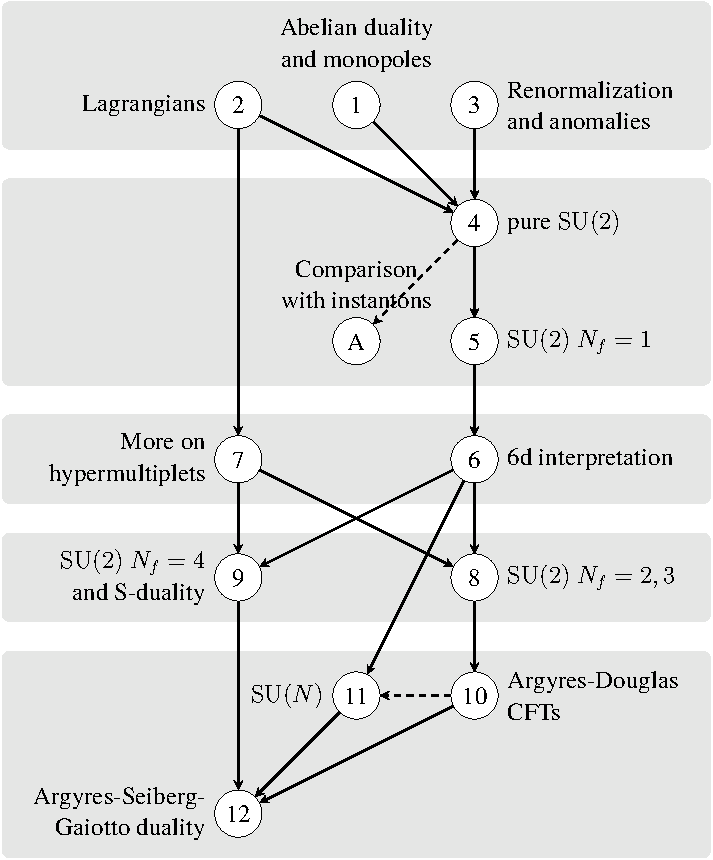
\includegraphics[width=12cm]{relation.pdf}
\caption{本讲义各节之间的依赖关系\label{fig:relation}}
\end{figure}

\section*{预备知识、免责声明与致谢}
\pdfbookmark[1]{预备知识、免责声明与致谢}{prerequisites}
读者需要能够熟练运用 $\cN{=}1$ 超场；我们在第\ref{sec:lagrangian}节约定所用记号。类似地，读者应当了解单圈重整化和微扰反常，并且至少听说过瞬子和单极子，尽管我们会作简短回顾并提供参考文献。本讲义不要求读者预先了解弦论或 M 理论，但读者应当愿意接受定义在维数高于四维的时空上的理论这一概念。除非另有说明，我们沿用物理学中的通常约定：凡是规范代数为 $\mathfrak{su}(N)$ 的规范群，都称为 $\SU(N)$，其他情形亦然。

拉格朗日量各项中的符号和 $i$ 的幂次并非完全一致或正确，但本讲义所呈现的总体思想应当没有问题。作者为使用同一个字母 $i$ 同时表示虚数单位和指标、使用同一个字母 $\theta$ 同时表示 $\theta$ 角和超坐标而致歉。总的来说，作者鼓励读者不仅阅读实际写出的内容，还要读出本来应当写出的内容。想必还存在许多其他排印错误、错误和有待改进之处。作者欢迎你提出任何意见，因此请不要犹豫，欢迎通过电子邮件 \href{mailto:[邮箱隐去]}{\texttt{[邮箱隐去]}} 与作者联系。

引文方面的不足最为明显，因为相关论文的数量极其庞大。作者非常确信，自己引用了过多自己的论文。除此以外，作者至少尝试提供一些近期论文的线索，使感兴趣的读者能够从这些论文的参考文献开始探索相关文献。作者也愿意在本讲义中增补参考文献，再次欢迎任何读者发来邮件。

本讲义根据作者 2011 年在名古屋大学和东北大学，以及 2013 年在立教大学的授课内容整理而成。作者感谢这三所大学的邀请者，使他有机会运用新的技巧综述 $\cN{=}2$ 超对称动力学。他也感谢这些课程的参与者在授课过程中提出的许多有益意见。作者研究这一主题的方法是在与诸多同事的讨论中形成的，并深受这些讨论的影响；本讲义中的大部分新论证，除那些错误的论证之外，都不应归功于作者。Ofer Aharony、Lakshya Bhardwaj、Chi-Ming Chang、Jacques Distler、Sheng-Lan Ko、John Mangual、Satoshi Nawata、Vasily Pestun、Futoshi Yagi 以及一位匿名审稿人，对本讲义初稿提出了有益意见。特别是 Simone Giacomelli、Brian Henning、Greg Moore、Tatsuma Nishioka、Jun'ya Yagi 和 Kazuya Yonekura，详细阅读了初稿，并向作者提出了许多改进建议。能够在此向他们致谢，令作者感到欣慰，也深感荣幸。最后，作者还要感谢 Teppei Kitahara 对插图制作提供的帮助；没有这些插图，本讲义将失去很大一部分价值。

作者还要感谢与其职位相伴的、分量恰到好处的各项职责：这些职责使他不再能够专心从事前沿研究，却仍然有一些时间来总结自己已经知道的内容。尤其要感谢他不得不参加的各种愚蠢的教师会议，本讲义的大部分插图就是在这些会议期间用笔记本电脑绘制的。因此，读者应当感谢东京大学盛行的过度官僚化体制，正是这一体制促成了本讲义的问世。本工作部分得到日本学术振兴会科学研究费补助金第 25870159 号项目资助，部分得到日本文部科学省 WPI 计划对东京大学 IPMU 的资助。
